\documentclass{report}
\usepackage[utf8]{inputenc}
\usepackage{geometry}
\usepackage{lipsum}
\usepackage{caption}
\usepackage{pgfplots}
\usepackage{booktabs}
\usepackage{relsize}
\usepackage{multicol}
\pgfplotsset{compat=1.18} % Imposta la compatibilità con pgfplots
\usepackage{mathtools}
\usepackage{amsmath}
\usepackage{enumitem}
\usepackage{array}
\usepackage{siunitx}
\usepackage[font=small,labelfont=bf]{caption}
\DeclareMathOperator\arctanh{arctanh}
\DeclareMathOperator\arcsinh{arcsinh}
\DeclareMathOperator\arccot{arccot}
\geometry{a4paper, top=2cm, bottom=2cm, left=2.5cm, right=2.5cm, bindingoffset=5mm}
\usepackage[italian]{babel}
\usepackage{dsfont}
\usepackage{amssymb}
\usepackage{graphicx}
\usepackage{wrapfig}
\usepackage{makecell}
\usepackage{tikz}
\usepackage{xfrac}
\usepackage{curve2e}
\usepackage{esint}
\usepackage{enumitem}

\def\width{180}
\def\height{260}
\definecolor{gridcolor}{RGB}{250,153,89}
%\definecolor{gridcolor}{RGB}{0,0,0}
\newcommand{\lapl}{\mathcal{L}}

\title{Ingegneria del Software}
\author{Francesco Mattone}


\begin{document}
\tableofcontents
\maketitle

\chapter{}
La MDA (Model Driven Architecture) è un processo di modellazione del codice basato sui diagrammi ottenuti tramite UP e UML.

\section{UML}
Linguaggio di modellazione usato in OOP.

\noindent
Unifica cicli di sviluppo, domini applicativi, processi di sviluppo con una struttura statica e un comportamento dinamico.

\smallskip
\noindent
Costituito da:
\subsection*{Diagrammi}
Sono 13 e modellano la struttura statica e dinamica, sono una vista del modello e lo strumento principale per aggiungere informazioni.
\subsection*{Vincoli}
Sono frasi di testo tra \{\} che definiscono una condizione/regola dell'elemento, che deve essere sempre vera.
\subsection*{Stereotipi}
Variazione di un elemento esistente che ha stessa forma ma diverso scopo.
\subsection*{Proprietà}
Qualsiasi valore associato ad un elemento di modellazione.

\noindent
Molti elementi hanno proprietà predefinite.

\subsection*{Etichette}
Informazioni aggiuntive da applicare agli elementi di modellazione o proprietà di nuovi elementi.

\section{UP}
\begin{itemize}
    \item \`E pilotato dai casi d'uso e dai fattori di rischio.
    \item \`E incentrato sull'architettura
    \item \`E iterativo ed incrementale
\end{itemize}

\newpage
\subsection*{Progetto}
Il progetto è diviso in:
\textbf{fasi}: il completamento di una fase ci fa raggiungere una \textit{milestone}.
\begin{itemize}
    \item \textbf{Avvio}: stabilire la fattibilità dei requisitifondamentali, business case e rischi critici.
    \item \textbf{Elaborazione}: baseline eseguibile, valutazionerischi, determinazione attributi di qualità, casi d'uso evalutazione risorse.
    \item \textbf{Costruzione}: terminare quanto fatto prima.
    \item \textbf{Transizione}: eliminare errori, creare sito utenti,adattare software al sito, manuale utente, consulenza utente,riepilogo.
\end{itemize}

\noindent
Ciascuna fase è formata da \textbf{iterazioni}: il completamento di un iterazione ci fa raggiungere una \textit{baseline}.
\begin{itemize}
    \item Pianificazione
    \item Analisi e progettazione
    \item Costruzione
    \item Integrazione e test
    \item Rilascio
\end{itemize}

\noindent
Ogni iterazione si compone di:
\begin{itemize}
    \item Requisiti
    \item Analisi 
    \item Progettazione 
    \item Implementazione 
    \item Test
\end{itemize}

\setcounter{chapter}{6}
\chapter{}
\section{Ciclo di vita}
\`E l'insieme delle attività ed azioni intraprese per realizzare un progetto software.
\subsection*{Cascata}

\begin{enumerate}
    \item \textbf{Studio di fattibilità}:

    \noindent
    I progettisti devono capire cosa vogliono i committenti.
    
    \noindent
    Stima di costi e tempi.

    \noindent
    Suddivisione progetto.

    \item \textbf{Fase di codifica}:
    
    \noindent
    Il progetto diventa un'unica entità su cui vengono svolti i test prestazionali.

    \item \textbf{Fase di manutenzione}:
    
    \noindent
    Dopo l'entrata in produzione, è la fase più costosa. Ci sono 3 tipi di manutenzione:
    \begin{itemize}
        \item \textit{Correttiva}: corregge errori nella progettazione.
        \item \textit{Adattiva}: aggiornare il sistema a cambiamenti esterni.
        \item \textit{Perfettiva}: caratteristiche aggiuntive.
    \end{itemize}

    \noindent
    Accquanto a queste ci sono 3 attività parallele:
    \begin{itemize}
        \item \textit{Produzione documentazione}
        \item \textit{Controllo qualità}
        \item \textit{Gestione processo}
    \end{itemize}
\end{enumerate}

\subsection*{Iterativo}
\`E il modello più efficace per la \textit{modifica} dei requisiti. Lo sviluppo avviene ripercorrendo un ciclo iterativo, ciò ci permette di sapere come agire in quella successiva.

\noindent
L'ordine di implementazione dipende dalle esigenze del progetto.

\noindent
Le iterazioni terminano una volta implementati tutti i requisiti.

\subsection*{Spirale}
\`E composta da 4 fasi:
\begin{enumerate}
    \item \textbf{Analisi}: Determinazione obiettivi e vincoli.
    \item \textbf{Progetto}: Valutazione alternative e identificazione rischi.
    \item \textbf{Sviluppo}: Codifica e test.
    \item \textbf{Collaudo}: Verifica operativa e pianificazione iterazione successiva.
\end{enumerate}

\noindent
La spirale è composta da anelli (dati da queste 4 fasi), al termine di ogni anello si avrà un'applicazione sempre più vicina a quella finale.

\noindent
Tra i vantaggi ci sono: riusabilità del codice, eliminazione progressiva degli errori, integra sviluppo e manutenzione.

\newpage
\section{Metodologie agili}
Pongono l'accento sulla \textbf{codifica}.

\noindent
Mantengono la fase di analisi in cui definiamo i requisiti.

\noindent
Passiamo all'implementazione di ogni singolo requisito, si assegna la responsabilità di un requisito ad un programmatore che se ne occuperà fino ai test.

\subsection*{Extreme programming}
Con questa metodologia si producono solo i semilatorati strettamente necessari, la produzione non è analizzata o pianificata a priori e il processo è un'insieme di attività da decidere di volta in volta.

\smallskip
\noindent
Il processo è formato da 4 attività: coding-testing-listening-design.

\noindent
Si assegnano a coppie di programmatori le \textit{userstory}. Le coppie vengono cambiate durante la progettazione per favorire la collettivizzazione del codice.

\noindent
I test vengono scritti prima del codice.

\subsection*{Scrum}
Si basa su 3 elementi fondamentali ed è diviso in sottoiterazioni di 24 ore:
\begin{enumerate}
    \item \textbf{Sprint}: Brevi iterazioni di 1 mese in cui vengono soddisfatti i requisiti. Alla fine si ottiene un semilavorato funzionante.
    \item \textbf{BackLog}

    \noindent
    Nel Backlog le funzionalità da soddisfare sono:
    \begin{itemize}
        \item \textit{Product}: relative al prodotto.
        \item \textit{Sprint}: relative allo sprint.
    \end{itemize}

    \item \textbf{Meeting}
    
    \noindent
    I meeting possono essere:
    \begin{itemize}
        \item Daily
        \item Sprint planning
        \item Sprint review
    \end{itemize}

    \noindent
    Nei meeting entrano in gioco 3 figure: product owner, scrum team, scrum master.
\end{enumerate}

\subsection*{Kanban}
\`E un sistema di gestione del flusso che si basa su 5 punti:
\begin{enumerate}
    \item \textbf{Visualizzare il flusso di lavoro}
    
    \noindent
    Scomponiamo il processo in fasi distinte e ne controlliamo l'avanzamento sulla \textbf{kanban board} grazie ai flussi di lavoro.

    \noindent
    La visualizzazione dei flussi si compone di 7 passi:
    \begin{enumerate}[label = \Roman*.]
        \item Identificare il flusso di valore
        \item Identificare ambito di lavoro
        \item Mappare le fasi del flusso di lavoro su colonne
        \item Definire i tipi di lavoro e cosa implica il "done"
        \item Decidere il modello di scheda per ogni tipo di lavoro
        \item Posizionare elementi di lavoro sulle carte
        \item Tracciare il flusso
    \end{enumerate}
    \item \textbf{Limitare il lavoro in corso}
    
    \noindent
    Assicurarsi il massimo flusso di un elemento dall'inizio alla fine.

    \noindent
    Ci sono 3 tipi di elementi nell'inventario: materie prime, lavori in corso e prodotti finiti.

    \item \textbf{Gestire e limitare il flusso}
    
    \noindent
    Kanbani  si concentra sull'assicurare un flusso di lavoro fluido con strumenti per individuare i bottleneck.

    \item \textbf{Esplicitare le politiche di processo}
    
    \noindent
    I processi ci dicono cosa fare, le politiche come farlo. Una buona pratica diventa un comportamento di routine ed aiuta i membri a mantenere il flusso.

    \item \textbf{Opportunità di miglioramento}
    
    \noindent
    Eliminazione dei vincoli in 5 passi:

    \noindent
    Identificarlo $\rightarrow$ Sfruttarlo $\rightarrow$ Sbordinare il lavoro $\rightarrow$ Elevarlo $\rightarrow$ Osservarne uno nuovo
\end{enumerate}

\subsection*{Scumban}
\`E un ibrido tra \textbf{scum} e \textbf{kanban} ma più allineato con quest'ultima.

\noindent
Non richiede che il product owner controlli il backlog poichè ci possono essere più stakeholder.

\noindent
Si pianifica il lavoro solo quando è necessario e si evitano le restrizioni temporali degli sprint.

\noindent
Il flusso è visualizzato sulle kanban card che permettono di dividere il lavoro in più fasi. 

\noindent
Gli elementi nelle colonne hanno priorità scelta dal team scrumban.

\subsection*{Devops}
Pratica che unisce il team \textbf{Dev} (sviluppo) con quello \textbf{Ops} (supporto) in modo da garantire una collaborazione fluida ed un miglior rilascio del software.

\noindent
I team possono concentrarsi unicamente sulla qualità e sulla velocità di consegna.

\medskip
\noindent
Si incoraggia all'eliminazione dei task manuali. Prima si sviluppa il codice a mano e lo si aggiorna nella repository, lo si genera e testa.

\subsubsection*{IaC}
Infrastructure as a Code - è una pratica in cui le infrastrutture sono configurate e gestite usando il codice non manuale.

\subsubsection*{Microservizi}
In questo tipo di architettura una singola app è un'insieme di piccoli servizi e componenti.

\subsubsection*{Topologie}
Il modo in cui DevOps viene applicato dipende dall'organizzazione. Ne esistono 9 topologie.
\begin{enumerate}
    \item \textbf{Collaborazion}: i team collaborano senza problemi.
    \item \textbf{Fully shared op's responsabilities}: i team OPS sono integrati negli altri.
    \item \textbf{OPS as Infrastructure as a Service}: hanno ancora un reparto ops.
    \item \textbf{As External Service}: non avendo un team ops delegano le loro mansioni ai dev.
    \item \textbf{Teams with an expiry date}: team temporaneo.
    \item \textbf{Advocacy team}: facilita la collaborazione tra dev e ops ricordando le pratiche.
    \item \textbf{SRE team}: team di Site Reliability Engineering che controlla che il lavoro dei dev sia conforme agli standard.
    \item \textbf{Container Driven Collaboration}: incapsulare i deployment e i requisiti in un contenitore. Rimuovere dipendenze tra dev e ops.
    \item \textbf{Dev \& Dba Collaboration}: i ruoli di specializzazione del database di entrambi i team sono integrati.
\end{enumerate}

\chapter{}
\section{Software come prodotto}
Caratteristiche del software:
\begin{itemize}
    \item Perminenza design
    \item Malleabilità
    \item Manutenzione correttiva e adattiva
    \item Qualità interna ed esterna
\end{itemize}

\noindent
Il rapporto che si crea tra committente e sviluppatore può essere di 4 tipologie:
\begin{enumerate}
    \item \textbf{Autoconsumo}: committente $\equiv$ produttore
    \item \textbf{Sviluppo interno}: committente = unità organizzativa distinta della stessa azienda
    \item \textbf{Sviluppo su commessa}: software house sviluppa prodotto dietro compenso. Il cliente può detenere per intero o parzialmente i diritti sul prodotto pagando di meno.
    \item \textbf{Software Shrink-Wrapped}: software house produce un suo prodotto.
\end{enumerate}

\noindent
La pianificazione dell'assegnazione delle risorse deve focalizzarsi nel punto minimo della curva non lineare:
$$E_N = \dfrac{D}{NS} + N\left[P+M(N-1)\right]$$
Dove:
\begin{itemize}
    \item $E_N$ = Tempo di rilascio
    \item $P$ = Overhead del signolo programmatore per la pianificazione del suo lavoro
    \item $M(N-1)$ = Overhead del singolo programmatore per la sincronizzazione con gli altri
    \item $S$ = Produttività
\end{itemize}

\subsection*{Costo del software}
Si usa il modello \textbf{CoCoMo} che distingue tra costi diretti ed indiretti.

\noindent
Entrano in gioco fattori organizzativi e dimensionali:
\begin{itemize}
    \item Numero di istruzioni
    \item Competenze dei programmatori
    \item Complessità del programma
    \item Stabilità dei requisiti
\end{itemize}

\noindent
La dimensione si determina con due possibili metriche:
\begin{itemize}
    \item \textbf{Metriche dimensionali}
    \item \textbf{Metriche funzionali}
\end{itemize}

\newpage
\noindent
La tecnica di stima dei costi parte da una caratteristica misurabile per predire lo sforzo di sviluppo ed i costi generali.

\noindent
La metrica dimensionale ha poco senso poichè non tiene conto della qualità del prodotto e del fatto che future modifiche potrebbero portare all'eliminazione di interi moduli.

\medskip
\noindent
CoCoMo2 è un modello previsionale per la stima dell'effort per un prodotto a partire dalla dimensione

\subsection*{Diagrammi di Gnatt}
Diagramma in cui l'asse delle ascisse indica il tempo e quello delle ordinate l'insieme dei task e sottotask che compongono il progetto. Tutto al fine di una corretta stima dei tempi di realizzazione dei task e delle risorse.

\subsection*{Function Point}
Misurano il software quantificando le funzionalità fornite verso l'esterno, basandosi sulla logica del sistema.

\noindent
La FPA (Function Point Analisis) è un processo semplice ma conciso, con 5 obiettivi:
\begin{enumerate}
    \item Valutare le richieste del cliente e quanto gli è stato fornito
    \item Metrica dimensionale per qualità e produttività
    \item Base per studi su prevenzione e stima
    \item Misurare software indipendentemente dalla tecnica di sviluppo
    \item Fattore di normalizzazione e raffronto con altre aziente
\end{enumerate}

\noindent
Esso inoltre fa riferimento a 3 principi fondamentali:
\begin{enumerate}
    \item \textbf{Misurare funzionalità richieste ed ottenute dai clienti}
    \item \textbf{Misurare manutenzione e sviluppo software}
    \item \textbf{Ottenere conteggio corrente tra pogetti ed organizzazioni}
    \begin{enumerate}
        \item Tipo di conteggio:
        \begin{itemize}
            \item Conteggio per sviluppo di progetto
            \item Conteggio per manutenzione evolutiva
            \item Conteggio applicativo
        \end{itemize}
        \item Ambito di conteggio e confini: per confini intendiamo la divisione tra una app e le altre. Per individuare i confini ci basiamo sulle funzionalità che l'utente può capire e descrivere.
        \item Function Type: componenti richiesti e visibili all'untente, dividiamo in:
        \begin{itemize}
            \item Funzioni dati
            \item Funzioni transazionali
        \end{itemize}
        \item Conteggio UFP: UFP = Funzioni Dati + Funzioni Transazionali
        \item Determinare VAF tramite caratteristiche generali del sistema:

        \noindent
        I Valve Adjustment Factor sono composti da $14$ caratteristiche dette GSC e sono usati per valutarne la complessità. Per tale valutazione si usa una scala di 6 valori (grado di influenza) ma per alcune GSC questo metodo cambia in quanto si assegna il punteggio in base alla presenza di sottocaratteristiche.

        \item FP: La loro individuazione avviene solo dopo il completamento dell'app.
    \end{enumerate}
\end{enumerate}

\newpage
\chapter{}
\section{Software coeme processo}
Vi sono 3 fasi principali:
\subsection*{1. Verifica}
Contronto tra il prodotto ottenuto e le specifiche richieste. Abbiamo 3 requisiti da verificare:
\begin{enumerate}
    \item I casi d'uso verificano i requisiti.
    \item Le classi sono in grado di fornire i casi d'uso.
    \item Il codice corrisponde alle classi che compongono il progetto.
\end{enumerate}

\noindent
La verifica va fatta ad ogni iterazione. Includiamo i "check di sanità" della compatibilità del codice e del fatto che compili senza errori.
\subsection*{2. Validazione}
Consiste nel coinvolgere i clienti ed avere il loro feedback alla fine di un'interazione.

\noindent
Per problematiche/incertezze/incompresioni conviene fare più iterazioni brevi.

\noindent
Il prodotto deve essere \textbf{intuitivo} e ciò può essere verificato da utenti esterni e/o esperti di usabilità.
\subsection*{3. Test}
Anche la fase di test è divisa in 3 parti:
\begin{enumerate}
    \item Trovare i bug
    \item Convincere il cliente che non ci sono bug
    \item Fornire informazioni sull'evoluzione del sistema
\end{enumerate}

\noindent
I testo sono generalmente divisi in 2 categorie:
\begin{itemize}
    \item \textbf{Test scatola nera}: funzionalità delle entità testate
    \item \textbf{Test scatola bianca}: struttura delle entità testate
\end{itemize}

\noindent
Affinchè il software sia percepito come di \textbf{alta qualità} dobbiamo:
\begin{enumerate}
    \item Testare l'intero sistema
    \item Verificare che continui a svolgere le funzioni supportate
    \item Testare i casi tipici anzichè limite
\end{enumerate}

\noindent
I test dovranno essere ripetibili, documentati, precisi ed eseguiti su software a configurazione controllata. Uno script può aiutare a eseguire un insieme di test, registrare i test effettuati, confrontare i valori.

\noindent
Lavorando ad oggetti, entrano in gioco altri concetti da considerare nello svolgimento dei test, tra cui:

\newpage
\begin{itemize}
    \item \textbf{Minima unità di test da considerare}

    \noindent
    In genere è preferibile pianifirare i test all'inizio dell'iterazione per evitare una progettazione affrettata.

    \item \textbf{Incapsulamento}:
    
    \noindent
    L'incapsulamento riduce il rischio di errori per comprensione errata delle interazioni tra componenti, ma rende difficile il test.

    \item \textbf{Polimorfismo}:
    
    \noindent
    L'ereditarietà ci aggiunge un nuovo livello di difficoltà poiché dovremmo testare tutte le funzionalità: è bene utilizzarlo se i vantaggi sono magggiori degli svantaggi.
\end{itemize}

\subsection*{Revisione e ispezione del codice}
Detto walkthrough, è un incontro in cui cerchiamo di identificare i problemi del prodotto.

\noindent
Sono noti come Formal Technical Review (FTR), si differenziano nei dettagli ma condividono 5 caratteristiche:
\begin{enumerate}
    \item I partecipanti sono allo stesso livello gerarchico
    \item L'artefatto è fornito in anticipo
    \item Agenda predefinita
    \item Non si discute su come rimediare agli errori
    \item La procedura successiva è atta alla risoluzione
\end{enumerate}

\subsection*{Manutezione}
Modifiche apportate ad un programma dopo la sua messa in uso.

\noindent
I tipi di manutenzione sono 4:
\begin{itemize}
    \item Perfettiva: 50\,\%
    \item Adattiva: 25\,\%
    \item Correttiva + Correttiva Emergenza: 21\,\%
    \item Preventiva: 4\,\%
\end{itemize}

\subsection*{Costi}
Sono legati soprattutto all'evoluzione del software e si dividono in base alla loro origine:
\begin{itemize}
    \item \textbf{Natura tecnica}:
    
    \noindent
    Complessità codice, cambiamenti linguaggi programmazione, cambiamenti infrastruttura, qualità formattazione.

    \item \textbf{Costo umano}:

    \noindent
    Stabilità team, responsabilità contrattuale, competenze personale.
\end{itemize}

\noindent
Terminologia:
\begin{itemize}
    \item \textbf{Manutenibilità}: facilità con cui un sistema può essere modificato.
    \item \textbf{Tracciabilità}: grado con cui si può stabilire una relazione tra due o più prodotti del processo di sviluppo.
    \item \textbf{Ripple Effect (catena)}: cambiamenti in una posizione del software possono provocare cambiamenti in altre posizioni.
    \item \textbf{Sistemi legacy}: sistema obsoleto usato in una azienta, la quale vuole disfarsene.
    \item \textbf{Analisi impatto}: processo con cui si identificano le conseguenze di un cambiamento sul resto del sistema.
\end{itemize}

\newpage
\noindent
La qualità del software dipende anche da quella dei suoi componenti. Distinguiamo 3 tipi di qualità che fanno riferimento:
\begin{itemize}
    \item \textbf{Interna}: alle proprietà rilevanti durante sviluppo e manutenzione.
    \item \textbf{Esterna}: alle proprietà che lo caratterizzano durante l'esecuzione.
    \item \textbf{In uso}: alle proprietà in uno specifico ambiente di esecuzione.
\end{itemize}

\subsubsection*{Riuso software}
\`E riconosciuto che un software migliore ha bisogno di un processo di progettazione basato sul riutilizzo del software.

\noindent
Questo viene fatto a diversi livelli:
\begin{itemize}
    \item Riuso sistemi
    \item Riuso app
    \item Riuso componenti
    \item Riuso oggetti e funzioni
\end{itemize}

\subsection*{Framework}
Sono entità moderatamente grandi che possono essere riutilizzate a metà strada tra il riutilizzo di sistemi e componenti.

\smallskip
\noindent
Il framework è il progetto di sottosistema composto da una collezione di classi astratte e concrete e le interfacce tra loro.

\noindent
Il sottosistema è implementato aggiungendo componenti per riempire parti del progetto ed istanziare le classi astratte nel framework.

\smallskip
\noindent
I \textbf{Web Application Framework} supportano la costruzione di siti web dinamici per tutti i tipi di linguaggi. Il modello di interazione è sul modello di progettazione composito \textbf{Model View Controller}.

\subsection*{Linee prodotto software}
Sono insiemi di applicazioni con architettura comune e componenti condivisi, ogni app è specializzata per soddisfare diversi requisiti.

\noindent
Include:
\begin{itemize}
    \item \textbf{Componenti di base}: danno supporto all'infrastruttura e non vengono modificati con una nuova istanza.
    \item \textbf{Componenti configurabili}: possono essere modificati e configurati per specializzarsi in una nuova app.
    \item \textbf{Componenti specializzati}: specifici nel dominio, possono essere sostituiti quando si ha un'istanza totalmente o parzialmente nuova.
\end{itemize}

\subsection*{Differenze tra Framework e Linee di Prodotto Software}
\subsubsection*{Framework}
\begin{itemize}
    \item Si basano su caratteristiche OOP come il polimorfismo.
    \item Si concentrano sulla fornitura di supporto tecnico.
\end{itemize}

\subsubsection*{Linee di Prodotto Software}
\begin{itemize}
    \item Non hanno bisogno di questo tipo di caratteristiche.
    \item Incorporano informazioni sul dominio della piattaforma.
    \item Controllano app per apparecchiature.
    \item Costituite da famiglie di app gestite dalla stessa organizzazione.
\end{itemize}

\newpage
\subsection*{Sistemi Applicativi Integrati}
Sono applicazioni che includono due o più sistemi applicativi, eventualmente legacy.

\noindent
Per svilupparli dobbiamo fare delle scelte di progetazione.

\noindent
L'integrazione si semplifica in presenza di un approccio orientato ai servizi che permette l'accesso alle funzionalità attraverso un'interfaccia standard.

\smallskip
\noindent
Alcune app possono offrire un'interfaccia di servizio che, però, a volte deve essere implementata dall'integratore di sistema.

\noindent
Si deve programmare un wrapper che nasconde l'app e fornisce servizi visibili dall'esterno.

\chapter{}
\section{Component based development paradigma}
Detto:
\begin{itemize}
    \item Component based software engineering - CBSE
    \item Component based development - CBD
\end{itemize}

\`E una branca dell'ingegneria del software che enfatizza la tecnica di suddivisione delle attività rispetto alle funzionalità disponibili.

\noindent
Si basa sul riutilizzo per definire, implementare e comporre componenti indipendenti liberamente accoppiate.

\subsection*{Componenti}
Sono piattaforme di partenza per l'orientamento ai servizi nel web service. Package, Moduli o Risorse Web che incapsulano funzioni, parliamo di Incapsulamento nei Componenti.

\begin{itemize}
    \item \textbf{Modulari e coesi}: processi collocati in componenti separati in modo che tutti i dati e le funzioni siano semanticamente correlati.
    \item \textbf{Sostituibili}: con una versione aggiornata o alternativa, senza arrecare danni al sistema dove operano.
    \item \textbf{Riusabili}: per essere riusabili, il software deve essere:
    \begin{itemize}
        \item Completamente documentato.
        \item Accuratamente testato.
        \item Robusto.
    \end{itemize}
\end{itemize}

\noindent
I componenti incapsulano sia le strutture dati sia gli algoritmi applicati ad essi.

\noindent
L'ingegneria basata sui componenti si basa anche sulla teoria precedente: architettura software, framework, design pattern, ecc\dots

\smallskip
\noindent
Un computer che esegue diversi componenti è detto \textbf{application server} e la loro combinazione è il calcolo distribuito.

\noindent
Un \textbf{component model} è una definizione di proprietà che i componenti devono soddisfare, nonché di metodi e meccanismi per la composizione dei componenti.

\subsection*{Distributed computing}
\`E una branca dell'informatica che studia i sistemi distribuiti ed i calcoli distribuiti, ovvero sistemi i cui componenti si trovano su diversi computer in rete, che comunicano tra loro per raggiungere un obiettivo comune.

\smallskip
\noindent
Si usa per risolvere problemi computazionali. Un problema viene diviso in molte task, ognuno risolto da uno o più computer comunicanti.

\newpage
\noindent
Questi sistemi possono essere caratterizzati da 2 tipi di calcolo:
\subsubsection*{Parallelo}
Tutti i processori possono avere accesso ad una memoria condivisa per scambiarsi informazioni e può  essere visto come una particolare forma accoppiata di calcolo.
\subsubsection*{Distribuito}
Ogni processore ha memoria distribuita e le informazioni sono date dallo scambio di messaggi.

\subsection*{Architetture}
Varie architetture hardware e software sono usate per il calcolo distribuito, con vari livelli:
\begin{itemize}
    \item \textbf{Basso livello}: è necessario interconnettere più cpu con qualche tipo di rete.
    \item \textbf{Alto livello}: è necessario interconnettere i processori in esecuzione nelle cpu con qualche tipo di sistema di comunicazione.
\end{itemize}

\noindent
La programmazione distribuita rientra in una delle seguenti \textbf{architetture}
\begin{enumerate}
    \item \textbf{Client-Server}: i client contattano il server per i dati.
    \item \textbf{Three-Tier}: spostano l'intelligenza del client su un livello intermedio in modo da utilizzarli senza stato.
    \item \textbf{N-Tier}: si riferiscono ad applicazioni web che inoltrano le loro richieste ad altri servizi aziendali.
    \item \textbf{Peer-To-Peer}: tutte le responsabilità sono equamente divise tra le macchine anche dette \textbf{peer}, esse fungono sia da client che da server.
\end{enumerate}

\noindent
Nel calcolo distribuito processi concorrenti comunicano tra loro attraverso protocolli, tipicamente in relazione \textbf{master-slave}.

\section{Service Oriented Architecture}
\`E uno stile che supporta all'orientamento ai servizi ed è applicata in quei casi in cui dei componenti forniscono servizi ad altri.

\noindent
\`E pensata per essere indipendente dai fornitori, prodotti e tecnologie.

\subsection*{Servizio}
\`E un'unità discreta di funzionalità a cui si può accedere da remoto e su cui possiamo agire ed aggiornare in modo \textbf{indipendente}.

\noindent
Ogni servizio ha 4 proprietà:
\begin{enumerate}
    \item Attività business ripetibile
    \item Autocontenuti
    \item \`E una scatola nera
    \item Può essere composto da altri servizi
\end{enumerate}

\noindent
Diversi servizi possono essere usati insieme come una rete per fornire le funzionalità di una grande app.

\medskip
\noindent
La SOA è supportata da terminologie e standard che facilitano la comunicazione e la cooperazione. Essa è legata al concetto di API (Application Programming Interface).

\newpage
\subsection*{Valori fondamentali delle SOA}
La SOA separa le funzioni in unità distinte, o servizi, che gli sviluppatori rendono accessibili su rete per permettere la combinazione e la riutilizzazione.

\noindent
Il manifesto delle SOA del 2009 prevede 6 valori fondamentali:
\begin{enumerate}
    \item Valore business
    \item Obiettivi strategici
    \item Servizi condivisi
    \item Interoperabilità intrinseca
    \item Flessibilità
    \item Perfezionamento evolutivo
\end{enumerate}

\subsubsection*{Principi}
Non ci sono standard relativi alla composizione di una SOA, ma dalle fonti pubblicate, in linea di massima, abbiamo:
\begin{enumerate}
    \item Contratto servizio standardizzato
    \item Autonomia riferimento del servizio
    \item Trasparenza posizione del servizio
    \item Longevità del servizio
    \item Astrazione del servizio
    \item Autonomia del servizio
    \item Apolidia del servizio
    \item Granularità del servizio
    \item normalizzazione
    \item Possibilità di comporli
    \item Scoperta del servizio
    \item Riutilizzabilità
    \item Incapsulamento
\end{enumerate}

\subsubsection*{Funzionamento}
Ogni building block può essere:
\begin{itemize}
    \item \textbf{Fornitore di servizi}: crea un sito web e fornisce le sue info al registro dei servizi.
    \item \textbf{Broker, registro o deposito servizi}: deve rendere le info riguardanti il servizio web disponibili a qualsiasi potenziale richiedente.
    \item \textbf{Richiedente/consumatore}: tramite i broker si legano ai fornitori per richiedere uno o più servizi.
\end{itemize}

\subsection*{Real Time Computing}
\`E il termine per indicare i sistemi hardware e software soggetti ad un vincolo di tempo indicati come deadline, dell'ordine dei millisecondi.

\noindent
L'elaborazione in tempo reale fallisce se non completata entro la scadenza specifica. Questo tipo di sistema controlla un ambiente ricevendo dati, elaborandoti e restituendo i risultati in modo sufficientemente rapido da influenzare l'ambiente in quel momento.

\newpage
\subsection*{Criteri}
Un sistema è in tempo reale se la correttezza totale di un'operazione dipende anche dal tempo in cui viene eseguita.

\noindent
Si classificano i sistemi in base alle conseguenze di una mancata deadline:
\begin{itemize}
    \item \textbf{Hard}: fallimento totale
    \item \textbf{Firm}: tollerabili, ma possono degradare la qualità del servizio, l'utilità diventa zero.
    \item \textbf{Soft}: tollerabili, ma possono degradare la qualità del servizio, l'utilità diventa zero dopo la deadline.
\end{itemize}

\chapter{Pattern}
\section{Pattern Architetturali}
Includono informazioni su quando il suo utilizzo è appropriato e i dettagli su vantaggi e svantaggi.

\subsection*{1. Model View Controller}
\`E la base per la gestione delle interazioni in molti sistemi web, supportato da molti linguaggi.

\noindent
Si basa sul principio di separazione delle responsabilità, il sistema è strutturato in 3 componenti logiche che interagiscono.

\begin{itemize}
    \item \textbf{Model}: si occupa dei dati del sistema e delle operazioni associate, quindi dello stato e della logica dell'applicazione.
    \item \textbf{View}: definisce e gestisce il modo in cui i dati sono presentati all'utente, quindi dell'interfaccia in risposta ad aggiornamenti del model.
    \item \textbf{Controller}: gestisce l'interazione degli utenti e traduce l'input in aggiornamenti passai al Model e View.
\end{itemize}

\noindent
\subsubsection*{Quando si usa?}
Quando ci sono più modi per visualizzare ed interagire con i dati e quando non sono noti i requisiti futuri di interazione e presentazione dati.

\subsubsection*{Vantaggi}
\begin{itemize}
    \item Rappresentazioni multiple della stessa informazione.
    \item Consente di modificare facilmente le interfacce utente.
    \item Consente di cambiare facilmente le risposte agli input dell'utente.
    \item Promuove il riuso.
    \item Consente agli sviluppatori di aggiornare simultaneamente interfaccia logica o input di un'app.
    \item Consente agli sviluppatori di focalizzarsi su un aspetto per volta.
\end{itemize}

\subsubsection*{Svantaggi}
\begin{itemize}
    \item Potrebbe richiedere altro codice o codice complesso per interazioni semplici.
\end{itemize}

\subsubsection*{Come funziona il ciclo?}
Sebbene le classi MVC siano separate, devono comunque comunicare regolarmente, pertanto ogni oggetto in MVC deve memorizzare un riferimento agli altri oggetti con cui interagisce.

\noindent
La comunicazione prevede una direzione attraverso i riferimenti:
\begin{enumerate}
    \item La view riceve l'input dall'utente e lo passa al controller.
    \item Il controller riceve l'input dell'utente dalla view.
    \item Il controller modifica il model in risposta all'input dell'utente.
    \item Il model cambia in base agli aggiornamenti del controller.
    \item Il model notifica i cambiamenti alla view.
    \item La view aggiorna l'interfaccia utente,.
\end{enumerate}

\subsubsection*{Responsabilità}
\textbf{Model}
\begin{itemize}
    \item Memorizza i dati e fornisce dei metodi specifici per definire i valori di questi dati e per recuperarli successivamente.
    \item I metodi di gestione dei dati non sono generici. Sono personalizzati per l'app e devono essere conosciuti al controller e alla view.
    \item I controller sono personalizzati per manipolare un model.
    \item I dati di un model possono essere cambiati da classi esterne o dalla propria logica interna.
    \item Il model deve poter far registrare le view.
    \item Se il model subisce un cambio significativo deve comunicarlo alle view.
    \item Il model implementa la logica del pattern MUC.
    \item Il model può fornire servizi di validazione dati.
\end{itemize}

\medskip
\noindent
\textbf{View}
\begin{itemize}
    \item Creare interfaccia utente e aggiornarla.
    \item Attendere cambiamenti dello stato del model.
    \item Passare gli eventi dell'input al controller.
    \item Non puà cambiare il model ma può chiedergli delle informazioni.
    \item Il cambiamento di una view si riflette sulle altre.
    \item La logica è centralizzata nel model, evitando duplicazioni di codice e modificando la view a runtime.
\end{itemize}

\medskip
\noindent
\textbf{Controller}
\begin{itemize}
    \item Si pone in attesa di notifiche dalla view e traduce gli input in cambiamenti del model.
    \item Interpreta opportunamente gli input prima di cambiare il model.
    \item Quando gli input non hanno effetti sul model esso istruisce la view per cambiare l'interfaccia.
\end{itemize}

\newpage
\subsection*{2. Layered Architecture}
\`E un altro modo di ottenere separazione ed indipendenza in quanto le funzionalità sono organizzate in strati separati che si basano sulle funzionalità ed i servizi dati dallo strato sottostante.

\subsubsection*{Descrizione}
Uno strato fornisce i servizi altro strato superiore, quindi quelli di livello più basso rappresentano i servizi base.

\noindent
Quest'architettura è modificabile e portabile; inoltre, se l'interfaccia non è modificata, un nuovo strato con funzionalità estese può sostituire uno esistente senza modificare altre parti del sistema.

\noindent
Se si modificano le interfacce di uno strato o si aggiungono funzionalità, ne risente solo quello adiacente.

\subsubsection*{Quando si usa}
Si usa:
\begin{itemize}
    \item Per costruire nuove funzioni per un sistema esistente.
    \item Quando lo sviluppo degli strati (e relative funzionalità) è distribuita su più team.
    \item Quando c'è una richiesta di protezione su più livelli.
\end{itemize}

\begin{multicols}{2}

    \subsubsection*{Vantaggi}
    \begin{itemize}
        \item Consente la sostituzione di interi strati se l'interfaccia non viene modificata.
        \item Le funzioni ridondanti possono essere fornite in ogni strato per aumentare la fidatezza.
    \end{itemize}
    
    \columnbreak
    
    \subsubsection*{Svantaggi}
    \begin{itemize}
        \item Difficile ottenere separazione netta degli strati.
        \item Le performance possono essere un problema a causa delle varie interpretazioni in quanto le richieste sono elaborate da ogni strato.
    \end{itemize}
    
\end{multicols}

\subsection*{3. Data Access Object}
Ha lo scopo di disaccoppiare l'accesso ai dati rispetto alla memorizzazione sottostante, consente di scegliere il tipo di DBMS da usare durante l'implementazione.

\noindent
Gli oggetti DAO consentono la portabilità dell'app da una sorgente dati all'altra, senza cambiare la logica business.

\medskip
\noindent
Portiamo un esempio di diagramma delle classi per il pattern DAO:
\begin{center}
    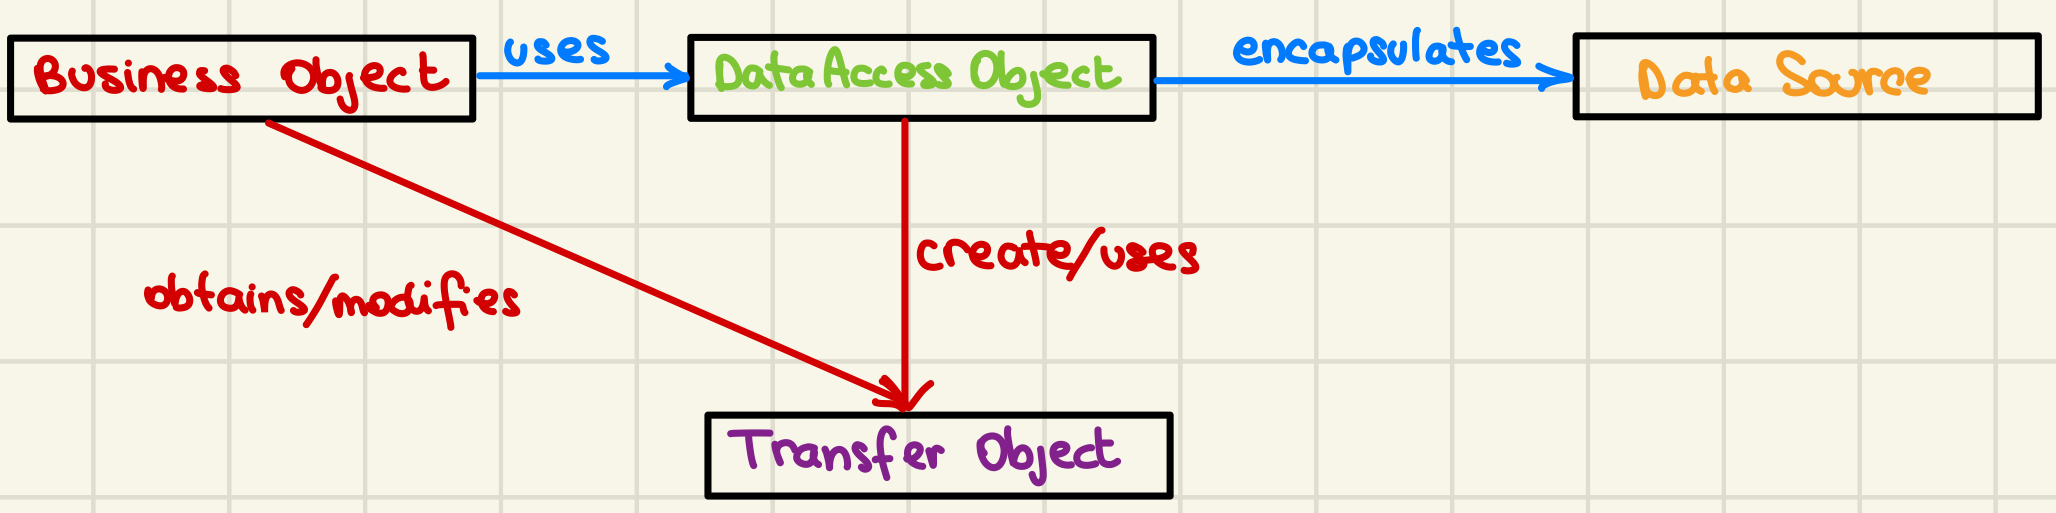
\includegraphics[width=0.75\textwidth]{immagini/IngSoft4.jpeg}    
\end{center}

\begin{itemize}
    \item \textbf{Business Object}: classe con la logica business che ha la responsabilità di specificare cosa e come modificare, non come memorizzare.
    \item \textbf{DataAccess Object}: nasconde la \textbf{Data Sources} effettiva.

    \noindent
    Una classe DataAccess Object può essere sostituita con un'altra se cambia la sorgente informativa.

    \item \textbf{Transfer Object}: viene usato per trasferire i dati da DataAccess Object a Business Object e viceversa. Rappresenta i dati nel Database e non è direttamente connesso a Data Source. Qualunque cambiamento a Transfer Object deve passare per DataAccess Object prima di diventare permanente.
\end{itemize}

\newpage
\subsection*{4. Repository}
Spiega come una serie di componenti interattivi possono condividere dati.

\subsubsection*{Descrizione}
Tutti i dati di un sistema vengono gestiti in un database centrare (repository) accessibile da tutti i componenti del sistema.

\noindent
I componenti interagiscono soltanto attraverso la repo.

\subsubsection*{Quando si usa?}
Si usa:
\begin{itemize}
    \item Quando nel sistema sono generati grandi volumi di informazioni che devono essere memorizzate per lungo tempo.
    \item Nelle applicazioni in cui i dati sono generati da un componente ed usati da un altro.
    \item Nei sistemi guidati dai dati, dove la loro inclusione nella repositori innesca l'azione/utilizzo di uno strumento
\end{itemize}

\begin{multicols}{2}

    \subsubsection*{Vantaggi}
    \begin{itemize}
        \item I componenti possono essere indipendenti.
        \item Le modifiche fatte da un componente possono essere rese note agli altri.
        \item Tutti i dati sono gestiti in modo coerente poichè si trovano nello stesso posto.
    \end{itemize}
    
    \columnbreak
    
    \subsubsection*{Svantaggi}
    \begin{itemize}
        \item La repository è un punto comune di malfunzionamento.
        \item Possono esserci inefficienze di organizzazione nella comunicazione con la repository.
        \item Può essere difficile distribuire le repository su più computer.
    \end{itemize}
    
\end{multicols}

\subsection*{5. Client-Server}
Illustra una tipica organizzazione a runtime di sistemi distribuiti.

\subsubsection*{Descrizione}
In questo tipo di architettura il sistema è presentato come un insieme di servizi, ciascuno dei quali è fornito da un server separato.

\noindent
I client sono utenti e accedono ai server per usufruire di tali servizi.

\subsubsection*{Quando si usa?}
Quando occorre accedere ai dati di un database da più postazioni. Poichè i server possano essere replicati, lo schema può essere utilizzato anche quando il carico su un sistema è variabile.

\begin{multicols}{2}

    \subsubsection*{Vantaggi}
    \begin{itemize}
        \item I server possono essere distribuiti in una rete.
        \item Le funzionalità comuni sono a disposizione di tutti i client.
        \item Le funzionalità comuni non devono essere implementate da tutti i servizi.
    \end{itemize}
    
    \columnbreak
    
    \subsubsection*{Svantaggi}
    \begin{itemize}
        \item Ogni servizio è un punto comune di malfunzionamento, soggetto a attacchi DOS e a guasti del server.
        \item Prestazioni imprevedibili, dipendenti da rete e da sistema.
        \item Problemi di gestione se i servizi sono di proprietà di più organizzazioni.
    \end{itemize}
    
\end{multicols}

\newpage
\subsubsection*{Come funziona il ciclo?}
I principali componenti di questo modello sono:
\begin{itemize}
    \item \textbf{Insieme di server} che offrono servizi ad altri sottoinsiemi.
    \item \textbf{Insieme di client} che richiedono i servizi offerti dai server.
    \item \textbf{Rete} che permette ai clienti di accedere ai servizi. 
\end{itemize}

\noindent
Le architetture sono di solito come architetture di sistemi distribuiti, ma il modello logico di servizi indipendenti eseguiti su server separati può essere implementato su un singolo dispositivo.

\subsection*{6. Pipe-and-Filter}
Rappresenta l'organizzazione a runtime di un sistema dove le trasformazioni funzionali elaborano i loro input e generano output.

\subsubsection*{Descrizione}
L'elaborazione dei dati del sistema è organizzata in modo che ciascun componente di elaborazione è discreto e svolge un particolare tipo di trasformazione dei dati.

\noindent
I dati fluiscono in un tubo (pipe) da un componente all'altro per essere elaborati.

\subsubsection*{Quando si usa?}
Nelle applicazioni per l'elaborazione dei dati (barch o basata su transazioni), dove gli input vengono elaborati in fasi separate per generare i relativi output.

\begin{multicols}{2}

    \subsubsection*{Vantaggi}
    \begin{itemize}
        \item Facile da capire e supporta il riutilizzo delle trasformazioni.
        \item Il flusso delle operazioni rispecchia la struttura di molti processi aziendali.
        \item Semplice evoluzione che permette di aggiungere trasformazioni.
        \item Può essere implementato come sistema sequenziale o parallelo.
    \end{itemize}
    
    \columnbreak
    
    \subsubsection*{Svantaggi}
    \begin{itemize}
        \item Il formato di trasferimento dei dati deve essere concordato.
        \item Ogni trasformazione deve leggere l'input e fornire l'output nel formato concordato.
        \item Aumentando così gli overhead del sistema e protrebbe rendere impossibile il riutilizzo dei componenti che usano strutture dati non compatibili.
    \end{itemize}
    
\end{multicols}

\subsubsection*{Come funziona il ciclo?}
I dati passano da una trasformazionne all'altra attraverso una sequenza ed ogni passo di elaborazione è implementato come trasformazione.

\noindent
I dati possono essere elaborati da ogni trasformazione elementare per elementi o in blocco.

\newpage
\section{Design Pattern}
Gli ingegneri del software hanno, nel corso del tempo, individuato delle best practice per la progettazione di software anche a livello di codice.

\noindent
I \textbf{Design Pattern} sono quindi dei pattern che specificano le linee guida sul progetto, ma a basso livello.

\noindent
In generale il pattern non rappresenta un algoritmo, ma una metodologia.

\noindent
Descrivendo un design pattern si forniscono delle voci che sono quasi sempre le stesse, ovvero:
\begin{enumerate}
    \item L'\textbf{intento} del pattern: descrizione del problema relativo al apttern e soluzione.
    \item La \textbf{motivazione}: spiegazione dettagliata del problema e della soluzione fornita.
    \item La \textbf{struttura delle classi}: mostra ogni parte del pattern e come queste sono legate.
    \item L'\textbf{esempio di codice}.
\end{enumerate}
    
\subsubsection*{Perché usarli?}
Rappresentano un toolkit di soluzioni provate e collaudate a problemi comuni e dunque insegnano a risolvere ogni tipo di problema utilizzando i principi della OOP.

\noindent
Vengono utilizzati per 3 motivi principali:
\begin{itemize}
    \item Risparmio di tempo.
    \item Permettono di scrivere codice standard.
    \item Supportano l'informatica del riutilizzo.
\end{itemize}

\medskip
\noindent
I design pattern sono 23 in totale divisi in 3 categorie:
\begin{itemize}
    \item \textbf{Pattern Creazionali}: hanno a che fare con la creazione di \textbf{istanze}.
    \item \textbf{Pattern Strutturali}: Hanno a che fare con la composizione di \textbf{classi} ed \textbf{istanze}.
    \item \textbf{Pattern Comportamentali}: Hanno a che fare con le inetrazioni di classi ed oggetti tra loro.
\end{itemize}

\section{Pattern Creazionali}
\subsection*{1. Factory Method}
Fornisce un'interfaccia per la creazione di oggetti in una superclasse, ma permette alle sottoclassi di modificare il tipo di oggetti che verranno creati.

\subsubsection*{Esempio pratico}
Abbiamo una app per la logistica. La prima versione si occupa solo dei camion, vogliamo incorporarci la logistica marittima; come facciamo per il codice? (Supponendo che la maggior parte del codice sia accoppiato alla classe "Truck").

\medskip
\noindent
Il pattern \textbf{factory} suggerisce di sostituire le chiamate dirette alla costruzione di oggetti (usando new) con chiamate ad uno speciale metodo factory.

\noindent
In questo modo possiamo \textbf{sovrascrivere} factory in una sottoclasse e cambiare la classe dei prodotti creati dal metodo, ciò è possibile solo se tali sottoclassi hanno in comune una superclasse o interfaccia.

\subsection*{2. Abstract Factory}
Consente di produrre linee di oggetti correlati senza specificarne le classi concrete.

\subsubsection*{Esempio pratico}
Simulatore di un negozio di mobili. Il nostro codice è costituito da classi che rappresentano: \textbf{famiglia} di prodotti e varianti di questa famiglia.

\newpage
\noindent
Vogliamo un modo per creare singoli oggetti d'arredo che si abbinino ad altri oggetti della stessa famiglia senza cambiare il codice esistente quando si aggiungono nuovi prodotti/famiglie.

\medskip
\noindent
Il patter abstract factory suggerisce di dichiarare esplicitamente le interfacce (chiamiamole interfacce 1) per ogni prodotto distinto della famiglia e fare in modo che tutte le varianti dei prodotti seguano quelle interfacce 1.

\noindent
Dichiariamo, a questo punto, l'Abstract Factory, un'interfaccia con un elenco di metodi di creazione per tutti i prodotti che fanno parte della famiglia. Tali metodi devono restituire i tipi di prodotti astratti rappresentati dalle interfacce 1.

\noindent
Per ogni variante di una famiglia creiamo una classe factory separata basata sull'Abstract Factory.

\medskip
\noindent
Una factory è una classe che restituisce prodotti di un particolare tipo, il \textbf{codice del client} deve operare sia con le fabbriche che con i prodotti in modo da permetterci di cambiare fabbrica e variante che gli si passa senza rovinare il codice.

\noindent
Gli oggetti concreti sono creati dall'app in fase di inizializzazione, poco prima dell'inizializzazione in se, l'app deve selezionare il tipo di factory a seconda della configurazione o delle impostazioni dell'ambiente.

\subsection*{3. Builder}
Costruire oggetti complessi passo dopo passo e produrre diversi tipi e rappresenzazioni di un oggetto usando lo stesso codice per la loro costruzione. Esso è utile quando si parla di customer massification, cioè massificare la personalizzazione dei prodotti rendendo ogni oggetto un assemblaggio completo di più oggetti.

\subsubsection*{Esempio pratico}
Pensiamo a come costruire un oggetto "House" che può essere una casa semplice o con più dettagli.

\noindent
Si potrebbero avere 2 approcci:
\begin{enumerate}
    \item Creare una sottoclasse per ciascuna variante ma avremmo un numero eccessivo di queste.
    \item Potremmo porre tutti i parametri delle varianti come attributi di "House" ma avremmo molti parametri "null" e chiamate dei costruttori brutte.
\end{enumerate}

\noindent
Il Pattern Builder suggerisce di estrarre il codice di costruzione dell'oggetto della propria classe e spostarlo in oggetti separati chiamati builder. Il pattern organizza la costruzione dell'oggetto in una serie di passi corrispondenti a metodi diversi.

\noindent
Per creare un oggetto si esegue una serie specifica di passi che cambia in base ai parametri desiderati.

\medskip
\noindent
I vari metodi possono essere dichiarati in un interfaccia e questa può essere implementata da diversi builder che costruiscono lo stesso oggetto in modo differente $\rightarrow$ il client deve conoscere i metodi a disposizione per ottenere quello che desidera.

\subsection*{4. Prototype}
Permette di copiare oggetti esistenti senza rendere il codice dipendente dalle loro classi, e quindi senza conoscerle in dettaglio.

\noindent
Supponiamo di avere un oggetto e volerne creare la copia esatta, dobbiamo considerare tutti i campi dell'oggetto originale e copiare i loro valori sul nuovo ma ciò a volte non possiamo farlo a causa della visibilità di alcuni campi.

\noindent
Un ulteriore problema è dato dal fatto che così facendo il codice diventa dipendente dalla classe dell'oggetto duplicato, inoltre capita di conoscere solo l'interfaccia che l'oggetto segue ma non la sua classe concreta.

\medskip
\noindent
Se il pattern Prototype suggerisce di delegare il processo di clonazione agli oggetti reali che vengono clonati, quindi dichiarare un'interfaccia comune per tutti gli oggetti che supportano la clonazione.

\noindent
L'implementazione di tale metodo semplicemente crea un oggetto della classe corrente e porta tutti i valori dei campi dal vecchio oggetto in quello nuovo, così facendo è l'oggetto originale ad auto-clonarsi.

\newpage
\subsection*{5. Singleton}
Consente di garantire che una classe abbia una sola istanza, fornendo un punto di accesso globale a tale istanza.

\medskip
\noindent
Il pattern Singleton risolve due problemi violando il principio della responsabilità unica.
\begin{itemize}
    \item \textbf{Assicurarsi che una classe abbia una sola istanza}

    \noindent
    Per controllare l'accesso a qualche risorsa condivisa. Quello che il pattern fa è che quando si vuole creare un nuovo oggetto, ma ne è già stato creato uno, ci restituisce quello già creato.

    \item \textbf{Fornire un punto di accesso globale all'unica istanza}
    
    \noindent
    Anzichè creare variabili globali per memorizzare oggetti essenziali, dove un qualsiasi codice può sovrascrivere il contenuto, possiamo accedere ad alcuni oggetti da qualsiasi punto del programma proteggendo l'istanza dalla sovrascrizione.
\end{itemize}

\noindent
Tutte le implementazioni del pattern Singleton hanno due passi in comune:
\begin{enumerate}
    \item \textbf{Rendere il costruttore privato} per evitare che altri oggetti lo chiamino.
    \item \textbf{Creare un metodo statico di creazione che funga da costruttore}: chiama il costruttore privato per creare un oggetto e salvarlo in un campo statico; così facendo tutte le successive chiamate a questo metodo restituiscono l'oggetto salvato nel campo statico che è sempre lo stesso.
\end{enumerate}

\section{Pattern Strutturali}
Riguardano le modalità con la quale classi ed oggetti vengono aggregati per formare entità più complesse.

\noindent
Ne esistono 2 categorie:
\begin{itemize}
    \item \textbf{Basati sugli oggetti}

    \noindent
    Descrivono le modalità di composizione di oggetti al fine di estendere in fase di esecuzione le funzionalità di una classe.

    \item \textbf{Basati sulle classi}

    \noindent
    Sfruttano l'ereditarietà multipla.
\end{itemize}

\subsection*{1. Adapter}
Consente la collaborazione di oggetti con interfacce compatibili.

\subsubsection*{Esempio pratico}
App per il monitoraggio del mercato aziendale che scarica vari dati in XML e li visualizza. Ad un certo punto decidiamo di migliorare l'app con librerie di analisi intelligente di terze parti, ma questa funziona solo con dati in formato JSON.

\smallskip
\noindent
Il patter Adapter suggerisce di creare un adattatore, speciale oggetto che converte l'interfaccia di un oggetto in modo che un altro possa capirlo mascherando gli oggetti, e quindi la complessità del tutto.

\noindent
La conversione usa 3 passaggi:
\begin{enumerate}
    \item L'adattatore definisce un'interfaccia compatibile con uno degli oggetti esistenti.
    \item Tramite l'interfaccia l'oggetto esistente può chiamare i metodi dell'adattatore.
    \item Alla ricezione di una chiamata, l'adattatore passa la richiesta al secondo oggetto, ma in un formato e ordine che esso si aspetta.
\end{enumerate}

\newpage
\subsection*{2. Bridge}
\`E un pattern strutturale che consente di suddividere una classe in due gerarchie che possono essere sviluppate indipendentemente l'una dall'altra.

\subsubsection*{Esempio pratico}
Supponiamo di avere una classe "Shape" avente due sottoclassi "Sphere" e "Cube". Immaginiamo di voler estendere questa gerarchia con colori per ogni forma.

\noindent
Avendo due sottoclassi si andranno a generare quattro combinazioni di sottoclassi. Volendo estendere ulteriormente andrebbe ad aumentare il numero di sottoclassi.

\noindent
Il problema nasce poichè vogliamo estendere le classi delle forme lungo due dimensioni indipendenti.

\medskip
\noindent
Il pattern Bridge suggerisce di passare l'ereditarietà alla composizione degli oggetti: significa che si estrae una delle dimensioni in una gerarchia di classe separata in modo che le classi originarie facciano riferimento ad un oggetto detta nuova gerarchia.

\medskip
\noindent
Tornando all'esempio, la classe Shape ottiene un attributo che si riferisce ad uno degli oggetti colore e questo riferimmento fungerà da ponte tra Shape e Color, quindi con questo pattern l'aggiunta di colori non richiederà di cambiare la gerarchia delle forme e viceversa.

\subsubsection*{Astrazione e Implementazione}
\begin{itemize}
    \item \textbf{Astrazione} (anche detta interfaccia)

    \noindent
    è uno strato di controllo ad alto livello per alcune entità che non deve svolgere alcun lavoro concreto da solo ma delegare il lavoro al livello di implementazione.

    \noindent
    Si considera GUI.

    \item \textbf{Implementazione} (anche detta piattaforma)
    
    \noindent
    Codice che lavora. Si considera API.
\end{itemize}

\subsection*{3. Composite}
Consente di comporre gli oggetti in strutture ad albero e poi lavorare con queste strutture come fossero singoli oggetti.

\subsubsection*{Esempio pratico}
Immaginiamo due tipi di oggetti "Product" e "Box", correlati tra loro dal fatto che una Box può contenere diversi Product e Box più piccole.

\noindent
Supponiamo di voler creare un sistema di ordini che utilizzi queste classi dove gli ordini possono riguardare prodotti semplici o box (per queste il prezzo totale si può trovare solo dopo averle scartate (approccio eccessivamente complesso)).

\medskip
\noindent
Il pattern Composite suggerisce di lavorare con Product e Box attraverso un'interfaccia comune che dichiara un metodo per calcolare il prezzo totale. Il più grande vantaggio è che non è necessario preoccuparsi delle classi di oggetti concreti che compongono l'albero, nel senso che non serve sapere se un oggetto è un prodotto o una box, è possibile trattarli egualmente attraverso l'interfaccia comune.

\subsection*{4. Decorator}
Permette di aggiungere nuovi comportamenti agli oggetti posizionandoli all'interno di speciali oggetti wrapper che contengono i comportamenti.

\subsubsection*{Esempio pratico}
Immaginiamo di lavorare ad una libreria di notifiche che permette ad altri programmi di notificare ai propri utenti eventi importanti.

\noindent
Inizialmente sviluppiamo una classe Notifier con compi campi, un costruttore ed un metodo $send()$.

\smallskip
\noindent
Se gli utenti desiderano ricevere notifica su Facebook e Slack potremmo estendere la classe Notifier con sottoclassi che abbiano metodi di notifica aggiuntivi. Se gli utenti volessero avere diversi tipi di notifica contemporaneamente dovremmo creare altre sottoclassi date dalle varie combinazioni, e il codice aumenterebbe eccessivamente.

\newpage
\noindent
Il pattern Decorator suggerisce di inserire un wrapper, ovvero un oggetto che può essere collegato a qualche oggetto target.

\noindent
Esso conterrà lo stesso insieme di metodi del target delegando ad esso le richieste che riceve, ma può alterare il risultato. Agli occhi del client i due oggetti sono identici.

\medskip
\noindent
Nell'esempio delle notifiche trasformiamo i metodi in decoratori, in questo modo il client dovrebbe avere un notificatore di base in un insieme di decoratori che corrispondono alle preferenze del cliente.

\subsection*{5. Facade}
Fornisce un'interfaccia semplificata per una libreria, un framework o qualsiasi altro insieme complesso di classi. Tale pattern è fondamentale con sistemi legacy.

\subsubsection*{Esempio pratico}
Immaginiamo di lavorare con un insieme di classi legato ad una sofisticata libreria o ad un framework. Normalmente si dovrebbero inizializzare tutti gli oggetti ed eseguire i metodi nell'ordine corretto. Così facendo la logica di business delle classi diventerebbe legata ai dettagli di implementazione delle classi di terze parti, rendendola difficile da comprendere e mantenere.

\medskip
\noindent
Il pattern Facade suggerisce di creare una classe facade che fornisce una semplice interfaccia ad un sottosistema complesso. Essa può fornire funzionalità limiitate rispetto a quelle del sottosistema integrale, ma ciò non risulta un problema dal momento che essa include le caratteristiche che interessano al client.

\subsection*{6. Flyweight}
Consente di inserire più oggetti nella quantità di RAM disponibile condividendo parti comuni dello stato tra più oggetti invece di mantenere tutti i dati in un oggetto.

\subsubsection*{Esempio pratico}
Supponiamo di aver creato un videogioco, uno sparatutto con una serie di particelle realistiche. Provandolo abbiamo notato che continua a bloccarsi dopo alcuni minuti a causa di RAM insufficiente.

\noindent
Il problema è legato alle particelle in quanto ognuna di queste è rappresentata da un oggetto contenente molti dati. Man mano che si va avanti con la partita, le nuove particelle non entrano più nella RAM causando il crash.

\medskip
\noindent
Controllando la classe Particle si nota che i campi Color e Spirit consumano molta più memoria rispetto ad altri, eppure sono dati quasi identici su tutte le particelle. Questi valori costanti prenderanno il nome di stato instrinseco, mentre il resto dello stato dell'oggetto, spesso alterato dall'esterno, è detto stato estrinsico.

\smallskip
\noindent
Il pattern Flyweight suggerisce di non memorizzare più lo stato estrinseco all'interno dell'oggetto, ma passare questo stato a metodi specifici che si basano su di esso.

\noindent
Un'oggetto che memorizza solo lo stato instrinseco si chiama Flyweight.

\subsection*{7. Proxy}
Consente di fornire un sostituto o un segnaposto per un altro oggetto. Un proxy controlla l'accesso all'oggetto originale, consentendo di eseguire qualcosa prima o dopo che la richiesta arrivi all'oggetto originale.

\subsubsection*{Esempio pratico}
Supponiamo di avere un oggetto massimo che consuma una grande quantità di risorse di sistema di cui abbiamo bisogno di tanto in tanto, ma non sempre.

\noindent
Una soluzione pigra potrebbe essere creare l'oggetto solo quando è necessario: tutti i client dovrebbero eseguire codice di inizializzazione differito. Questo causerebbe tantissime duplicazioni.

\medskip
\noindent
Il pattern Proxy suggerisce di creare una nuova classe proxy con la stessa interfaccia di un oggetto di servizio originale. In questo modo si può aggiornare l'app in modo che passi il proxy a tutti i client dell'oggetto originale.
Al ricevimento di una richiesta da parte di un client, il proxy crea un oggetto di servizio reale e delega ad esso tutto il lavoro.

\noindent
Il vantaggio sta nel fatto che il proxy può essere passato a qualsiasi client che si aspetta un oggetto di servizio reale.

\section{Pattern Comportamentali}
Si riferiscono alla distribuzione delle responsabilità di oggetti correlati tra loro.

\noindent
Si focalizzano sulle modalità di comunicazione e collaborazione tra oggetti e classi fornendo una soluzione per incapsulare le diverse funzionalità in un oggetto specifico con l'intento di delegare ad esso l'esecuzione del codice vero e proprio.

\smallskip
\noindent
Esistono due categorie di pattern comportamentali:
\begin{itemize}
    \item \textbf{Behavorial class pattern} (usano l'ereditarietà)
    \item \textbf{Behavorial object pattern} (usano la composizione)
\end{itemize}

\subsection*{1. Chain of Responsability}
Consente di passare le richieste lungo una catena di gestori. Al ricevimento di una richiesta ogni gestore decide di elaborare la richiesta oppure passarla al successivo gestore della catena.

\subsubsection*{Esempio pratico}
Immaginiamo di lavorare ad un sistema di ordini online. Vogliamo limitare l'acceso al sistema così che solo gli utenti autenticati possono creare ordini. Questi controlli devono essere eseguiti in sequenza.

\noindent
Una volta aggiunti i controlli sequenziali il codice di questi si gonfia sempre di più, inoltre la modifica di un controllo può influire sugli altri.

\medskip
\noindent
Il patter Chain of Responsability si basa sulla trasformazione di particolari comportamenti in oggetti standalone chiamati handler, nel nostro esempio ogni controllo dovrebbe essere associato ad una propria classe.

\noindent
Il pattern suggerisce di collegare questi gestori in una catena dove ogni gestore ha un campo per memorizzare un riferimento al gestore successivo nella catena. Un gestore può decidere di non passare la richiesta ulteriormente nella catena e fermare qualsiasi ulteriore elaborazione.

\smallskip
\noindent
\`E fondamentale che tutte le classi degli handler implementino la stessa interfaccia. Inoltre ogni handler concreto dovrebbe preoccuparsi solo di quello seguente che ha un metodo \textit{execute()}, in questo modo si possono comporre catene a runtime senza accoppiare il codice alle loro classi complete.

\subsection*{2. Command}
Trasforma una richiesta in un oggetto a se stante che contiene tutte le informazioni sulla richiesta. Tale trasformazione permette di parametrizzare i metodi con diverse richieste, ritardare o mettere in coda l'esecuzione di una richiesta e supportare le operaizoni annullabili.

\subsubsection*{Esempio concreto}
Lavoriamo ad un nuovo text editor. Dobbiamo creare una barra degli strumenti con una serie di pulsanti. Creiamo una classe Button che può essere utilizzata sia per la barra degli strumenti che per altri pulsanti generici. Si suppone che tutti questi pulsanti facciamo cose diverse e quindi dobbiamo capire dove posizionare il codice per i vari gestori.

\medskip
\noindent
Una buona gestione si basa sul principio di separazione dei problemi, cioè struttura di una app in strati.

\noindent
Il pattern Command suggerisce che gli oggetti GUI non dovrebbero inviare queste richieste direttamente, ma dovrebbero estrarre tutti i dettagli della richiesta in una classe command separata, con un metodo che inneschi tale richiesta. I command servono come collegamenti tra le varie GUI e gli oggetti della logica di business. Così la GUI si occupa di attivare il comando.

\noindent
Dobbiamo poi fare in modo che i comandi implementino la stessa interfaccia che solitamente ha un singolo metodi di esecuzione che non accetta parametri e permette di utilizzare vari comandi con lo stesso mittende della richiesta, senza accoppiarlo a classi concrete di comandi.

\smallskip
\noindent
Tornando all'editor di testo, dopo aver applicato il pattern Command è sufficiente mettere un singolo campo nella classe base Button che memorizza un riferimento ad un oggetto di comando.

\newpage
\subsection*{3. Iterator}
Permette di attraversare gli elementi di una collezione senza esporre la rappresentazione sottostante.

\subsubsection*{Esempio pratico}
Le collezioni sono uno dei tipi di dati più utilizzati nella programmazione. La maggior parte delle collezioni memorizza i propri elementi in semplici liste. Ma per accedere ad essi serve un metodo veloce che si complica quando abbiamo a che fare con una struttura dati complessa (come quella ad albero) anche perche queste possono essere attraversate in vari modi.

\noindent
Quindi per soddisfare criterio di attraversamento bisognerebbe implementare algoritmi diversi.

\medskip
\noindent
L'idea del patter Iterator è quella di estrarre il comportamento di attraversamento di una collezione in un oggetto chiamato Iteratore.

\noindent
L'oggetto Iteratore si occupa di implementare l'algoritmo di attraversamento a tutti i dettagli dello stesso, come la posizione corrente, il numero di elementi rimanenti, ecc\dots

\noindent
La presenza di tali dati consente di far attraversare la stessa collezione da più iteratori nello stesso momento, quindi quando un iteratore ha concluso il suo attraversamento non restituisce più nulla.

\noindent
Tutti gli iteratori devono implementare la stessa interfaccia in modo da rendere il codice del client compatibile con qualunque tipo di collezione o con qualsiasi algoritmo di attraversamento.

\subsection*{4. Mediator}
Consente di ridurre le interdipendenze tra gli oggetti. Il pattern inserisce un mediatore che si occupa di far comunicare tra loro i vari oggetti solo passando attraverso di lui.

\subsubsection*{Esempio pratico}
Supponiamo di avere una finestra GUI per gestire i profili dei clienti. Questa finestra è composta da vari elementi che possono interagire tra loro, questo gran numero si concretizza in altrettante classi che devono avere riferimenti agli altri elementi della finestra.

\noindent
Così facendo oltre ad avere un codice caotico non si possono riutilizzare quelle classi in altre parti del codice visto che possiedono riferimenti che potrebbero non servire.

\medskip
\noindent
Il pattern Mediator suggerisce di interrompere ogni comunicazione diretta tra i componenti che si desidera rendere indipendenti l'uno dall'altro. I componenti dovranno invece collaborare indirettamente, chiamando uno speciale oggetto mediatore che reindirizza le chiamate ai componenti appropriati, quindi in questo modo i componenti dipenderanno da una singola classe mediatore, evitando i multipli riferimento alle altre classi in ognuno di essi.

\noindent
Per semplificare questo processo è buona pratica inserire un interfaccia comune a tutti gli elementi e faccia da tramite per comunicare con il mediatore.

\subsection*{5. Memento}
Permette di salvare e ripristinare lo stato precedente di un oggetto senza rivelare i dettagli della sua implementazione.

\subsubsection*{Esempio pratico}
Immaginiamo di creare un text editor. Vogliamo consentire che gli utenti annullino le operazioni effettuate sul testo. Decidiamo di usare l'approccio diretto: prima di ogni operazione l'app registra lo stato di tutti gli oggetti e lo salva da qualche parte nella memoria.

\noindent
Quando un utente vuole tornare indietro di una azione l'app recupera questa istantanea e la usa per ripristinare lo stato di tutti gli oggetti.

\noindent
Analizzando questo approccio, è immediato rendersi conto del fatto che causerebbero delle problematiche:
\begin{enumerate}
    \item Servirebbero tantissime chiamate a metodi per ottenere i valori degli attributi quando salviamo l'istantanea.
    \item Aggiungendo altre classi bisognerebbe modificare anche le classi responsabili della copia dello stato.
    \item Si metterebbero a rischio la sicureza dell'app rendendo accessibili a tutti i dati copiati.
\end{enumerate}

\newpage
\noindent
Il pattern Memento delega la creazione degli Snapshot dello stato all'oggetto stesso che deve essere fotografato.

\noindent
\`E l'oggetto stesso che si occupa di copiarsi. Il pattern suggerisce di memorizzare, poi, la copia dello stato dell'oggetto in un oggetto speciale chiamato Memento. Il suo contenuto non è accessibile a nessun altro oggetto se non a quello che lo ha prodotto.

\noindent
Infatti, altri oggetti devono comunicare con i memeto utilizzando un'interfaccia limitata che può permettere di recuperare i metadati dello snapshot, ma non lo stato dell'oggetto originale.

\subsection*{6. Observer}
Permette di definire un meccanismo di sottoscrizione per notificare a più oggetti gli eventi che accadono all'oggetto che stanno osservando.

\subsubsection*{Esempio pratico}
Immaginiamo che un cliente sia interessato ad un nuovo prodotto e sia in attesa del suo rilascio. Il cliente potrebbe visitare il negozio ogni giorno per verificare la disponibilità. Ma la maggior parte di questi viaggi sarebbe inutile. In alternativa il negozio potrebbe inviare email a tutti i clienti, ma questo sconvolgerebbe altri clienti non interessati al prodotto.

\medskip
\noindent
Il pattern Observer offre una soluzione molto semplice a livello logico: chi è interessato (subscriber) al cambiamento dell'oggetto interessante (detto subject o publisher) si iscrive ad una lista in modo tale che il publisher, cambiando stato, mandi una notifica dell'avvenimento a tutti i subscriver iscritti a una lista. Al livello di implementazione il pattern suggerisce di aggiungere un meccanismo di sottoscrizione alla classe del publisher in modo che i singoli oggetti possano iscriversi o cancellarsi da un flusso di eventi provenienti da quel publisher.

\noindent
Così, ogni volta che un evento importante accade al publisher individua i suoi subscriber e chiama il metodo di notifica specifico sui loro oggetti.

\subsection*{7. State}
Permette ad un oggetto di modificare il suo comportamento quando il suo stato interno cambia.

\subsubsection*{Esempio pratico}
Immaginiamo di avere una classe Document. Un documento può essere in uno di tre stati: Draft, Moderation e Published.

\noindent
Vogliamo che il metodo \textit{publish()} del documento funziona in modo diverso in base allo stato in cui si trova l'oggetto: 
\begin{itemize}
    \item In Draft sposta il documento alla moderazione.
    \item In Moderation rende il documento pubblico.
    \item In Published non fa nulla.
\end{itemize}

\noindent
Per implementare questo comportamento dovremmo usare una serie di costrutti \textit{if-elif} ma volendo aggiungere altri stati il codice crescerebbe a dismisura.

\medskip
\noindent
Il pattern Stage suggerisce di creare nuove classi per tutti i possibili stati di un oggetto e di estrarre tutti i comportamenti specifici dello stato in queste classi. In questo modo invece di implementare tutti i possibili comportamenti da solo, l'oggetto originale memorizza un riferimento a uno degli oggetti di stato che rappresenta il suo stato corrente e delega il lavoro relativo allo stato di quell'oggetto, il tutto tramite un'interfaccia comune.

\subsection*{8. Strategy}
Permette di definire una famiglia di algoritmi, di mettere ciascuno di essi in una classe separata e di rendere i loro oggetti intercambiabili.

\subsubsection*{Esempio pratico}
Supponiamo di sviluppare una app che utilizza moltissime collezioni per memorizzare i dati. Immaginiamo di aver bisogno di ordinare spesso queste collezioni.

\noindent
Abbiamo a disposizione diversi algoritmi di ordinamento ma ognuno di questi si comporta in modo diverso in base alle situazioni e non necessariamente quello più efficiente nella media è ugualmente il più efficiente in una situazione specifica, quindi dobbiamo trvare l'algoritmo giusto.

\medskip
\noindent
Il pattern Strategy suggerisce di prendere una classe che fa qualcosa di specifico in molti modi diversi ed estrarre tutti questi algoritmi in classi separate chiamate Strategie. La classe originale deve avere un campo per memorizzare un riferimento ad una delle strategie in modo da delegare il lavoro ad un oggetto strategia invece di eseguirlo da solo.

\noindent
Così facendo la classe originale non è responsabile della selezione di un algoritmo ma è il client a passare la strategia desiderata alla classe originale.

\noindent
Anche qui l'interfaccia generica ha un ruolo centrale, quindi l'interfaccia esponde solo un singolo metodo per l'attivazione dell'algoritmo incapsulato nella strategie selezionata.

\subsection*{9. Template Method}
Definisce lo scheletro di un algoritmo nella superclasse ma lascia che le sottoclassi sovrascrivano specifici passi dell'algoritmo senza modificarne la struttura.

\subsubsection*{Esempio pratico}
Immaginiamo di creare un app di data mining che analizza dei documenti aziendali dai vari formati da cui estrarre i dati significativi in un formato uniforme. Si potrebbe creare una classe per ogni formato ma avrebbero un codice simile.

\noindent
Vogliamo dunque eliminare la duplicazione lasciando intatta la struttura dell'algoritmo.

\medskip
\noindent
Il pattern Template Method suggerisce di suddividere un algoritmo in una serie di passi, trasformarli in metodi separati ed inserire una serie di chiamate a questi metodi all'interno di un singolo template method. I passi possono essere astratti o avere un'implementazione predefinita.

\noindent
Per utilizzare l'algoritmo si presuppone che il client debba fornire la propria sottoclasse, implementare tutti i passi astratti e, se necessario, sovrascrivere gli opzionali.

\medskip
\noindent
Ci sono 2 tipi di passi:
\begin{itemize}
    \item \textbf{Astratti}: devono essere implementati da ogni sottoclasse.
    \item \textbf{Opzionali}: hanno qualche implementazione di default ma possono essere sovrascritti.
\end{itemize}

\noindent
Esiste un'ulteriore passo detto Hook, opzionale con un corpo vuoto, ovvero un metodo ne implementato ne astratto. Un Template Method funzionerebbe anche se un hook non viene sovrascritto.

\subsection*{10. Visitor}
Consente di separare gli algoritmi dagli oggetti su cui operano.

\subsubsection*{Esempio pratico}
Immaginiamo di sviluppare un'app che funzioni con informazioni geografiche strutturate come un grafo, Ogni nodo del grafo rappresenta un'entità della citta. Al livello di codice \textbf{tipo di nodo = classe} e \textbf{specifico nodo = oggetto}.

\noindent
Se avessimo la necessità di esportare il tutto in formato XML potremmo pensare di aggiungere un metodo di esportazione ad ogni classe nodo, ma ciò potrebbe causare problemi nel caso volessimo un diverso formato di esportazione.

\medskip
\noindent
Il pattern Visitor suggerisce di collocare il nuovo comportamento in una classe separata chiamata Visitor, invece di integrarlo nelle esistenti.

\noindent
L'oggetto originale viene passato ad uno dei metodi del visitor come argomento, fornendogli l'accesso ai dati contenuti nell'oggetto.

\noindent
Anche qui si estrae un'interfaccia comune per tutti i visitor per permettere ai modi di lavorare con ogni nuovo visitor introdotto.






 \end{document}